\documentclass{llncs}
\usepackage[czech]{babel}
\usepackage[utf8]{inputenc}
\usepackage{graphicx}
\usepackage{amssymb}
% for example: \labeldest{oo}{\chapter{Anal�za a n�vrh}}
\def\labeldest#1#2{
  \ifx\pdfoutput\nodefined
  \else
    \pdfdest name {#1} fitbh
  \fi %
  #2 
  \label{#1}
}

% for example: \reflink{kapitole}{oo}
\def\reflink#1#2{%
\ifx\pdfoutput\nodefined%
\else%
\pdfstartlink goto name {#2}%
\fi %
#1~\ref{#2}%
\ifx\pdfoutput\nodefined%
\else%
\pdfendlink%
\fi%
}

% for example: \image{img_tridni}{Popis}{img/class}{16cm}{20cm}
\def\image#1#2#3#4#5{
  \begin{figure}[htb]
  \begin{center}
    \ifx\pdfoutput\undefined
       \includegraphics[width=#4,height=#5]{#3.eps}
    \else
      \pdfximage width #4 height #5 {#3.pdf}
      \mbox{\pdfrefximage \pdflastximage}
    \fi
  \end{center}
  \caption{#2}
  \label{#1}
\end{figure}}

% for example: \image{img_tridni}{Popis}{img/class}{16cm}{20cm}
\def\imagejpg#1#2#3#4#5{
  \begin{figure}[htb]
  \begin{center}
    \ifx\pdfoutput\undefined
       \includegraphics[width=#4,height=#5]{#3.eps}
    \else
      \pdfximage width #4 height #5 {#3.jpg}
      \mbox{\pdfrefximage \pdflastximage}
    \fi
  \end{center}
  \caption{#2}
  \label{#1}
\end{figure}}

\newcounter{ExampleCount}
\setcounter{ExampleCount}{0}

\newcounter{DefinitionCount}
\setcounter{DefinitionCount}{0}



\title{Synchronizace a replikace geodat v prostředí Esri platformy}
\author{Markéta Solanská}
\institute{Katedra geoinformatiky, Přírodovědecká fakulta, Univerzita Palackého v Olomouci, 17. listopadu 50, 779 00 Olomouc, Česká republika, \\
\email{marketa.solanska@gmail.com}} 

\begin{document}
\maketitle

\begin{abstract}
  Tato práce hodnotí možnosti dostupných replikačních řešení a na základě toho
  navrhuje databázové řešení s ohledem na možnosti a požadavky katedry. V
  rešerší části byly vymezeny pojmy synchronizace, replikace a související
  pojem verzování a popsána replikace včetně variant synchronní, asynchronní,
  jednosměrné, obousměrné, kaskádové, logické i fyzické. Byly rozebrány
  požadavky na databázové ukládání dat jednotlivých produktů ArcGIS a byla
  podrobně popsána technologie ArcSDE, která se v ArcGIS produktech používá pro
  připojení k databázi. Na základě rešerše byl vybrán databázový systém
  PostgreSQL, který je možno použít v kombinaci s produkty ArcGIS, což bylo
  jedním z hlavních požadavků pro výběr databázového systému. Byl sestaven
  návrh databázového řešení, který zohledňuje všechny požadavky katedry a
  možnosti daných technologií. Bylo vytvořeno testovací prostředí na serveru
  poskytnutém katedrou, na němž byly dané procesy otestovány. Na základě toho
  byl pak sepsán podrobný popis toho, jak nastavit replikaci ve variantě
  streaming a Slony-I. Návrh zahrnuje také možnost použití nástroje pgpool pro
  rozložení zátěže mezi servery v databázovém clusteru.
\end{abstract}


\begin{keywords}
  replikace, synchronizace, verzování, databázový systém, Po\-stgreSQL, ArcSDE, ArcGIS
\end{keywords}

\begin{abstractEnglish}
  The main goal of this thesis is to evaluate options of replication solutions
  which are available and based on this research design a~database solution
  which considers possibilities and requirements of the Department of
  Geoinformatics. In the theoretical part terms replication, synchronization
  and versioning are defined including description of synchronous,
  asynchronous, master-slave, multimaster, cascade, logical and physical
  replication. The requirements of ArcGIS products for storage of data in
  database were considered and ArcSDE Technology which is used by ArcGIS
  products for database storage of spatial data was described. Based on the
  research database management system PostgreSQL was chosen because it is
  supported by ArcGIS products. The design of the database solution was created
  based on all requirements and the main processes were tested. Based on that a
  manual of the proposed replication solution setup was written. Two
  replication options were tested - PostgreSQL native streaming replication and
  replication using PostgreSQL extension Slony-I. The design includes a
  description of usage of pgpool utility used for load-balancing. 
\end{abstractEnglish}

\begin{keywordsEnglish}
  replication, synchronization, versioning, database management system, PostgreSQL, ArcSDE, ArcGIS
\end{keywordsEnglish}

Dnešní trend je ukládat a ponechávat stále více dat pouze v digitální podobě. Mnoho dokumentů už se vůbec netiskne do papírové podoby, což podporuje i trend e\-le\-ktro\-nic\-kých schránek a podpisů. S přibývajícím množstvím dat je však třeba řešit komplikace, které informace uložené pouze v elektronické podobě přinášejí. Počítačoví experti řeší například otázky, kam ukládat tak velké množství dat, jak data efektivně aktualizovat, jak zabránit poškození dat ať už způsobených lidským faktorem či chybou hardware. V případě, že se poškodí disk, můžeme často během okamžiku přijít o~všechna data, někdy však pro ztrátu dat stačí pouze stisknout tlačítko na klávesnici.

Dnes je běžné, že má každý hned několik internetových účtů pro přihlášení do banky, pojišťovny, různých internetových obchodů, či sociální sítě. Často však, například z důvodu přetížení, nastávají problémy s pomalým připojením nebo úplnou nedostupností zvolené služby. I to jsou problémy, které velké množství dat a vysoký počet uživatelů přináší. Jak tedy pracovat s těmito objemy, jak zabránit komplikacím, které mohou poškodit či zcela zničit celou dosavadní práci, a~jak zrychlit celý proces práce s daty? 

Řešením velkého počtu výše uvedených problémů může být ukládaní dat do databáze a jejich následná replikace. Replikací je myšlena pokročilá funkcionalita, která zajišťuje kopii dat na více serverů. Nabízí ji většina dnešních databázových serverů, zajišťuje větší robustnost databáze a vysokou dostupnost dat. Replikaci lze využít ve všech odvětvích, která pracují s daty. Výjimkou není ani geoinformatika, která často pracuje s~velkými objemy dat, které nesou informaci o geografické poloze. Právě reprezentace geografické polohy, skrze textový zápis souřadnic daných bodů, může způsobit razantní zvýšení objemu dat. U webových map se musí řešit velký počet dotazů do databáze, protože například každé posunutí výřezu či přiblížení, resp. oddálení výřezu mapy, je samostatným dotazem, který musí kapacita serveru zvládat. Například pokud bude uživatel procházet plánovanou 100km trasu posouváním výřezu mapy po 10~km, může to serveru způsobit velkou zátěž.

Data středně velkého až velkého projektu je vhodnější ukládat do databáze než jiných formátů typu shapefile, GML nebo obyčejného tabulkového procesoru. Nabízí nám to sofistikované uložení dat, propojení jednotlivých vrstev a připojení atributů ke geometrii, snadnou přenostitelnost dat i efektivní vyhledávání. Replikace samotná se poté využívá pro zajištění kopie dat a následnou aktualizaci změn, která v databázi nastanou. 

Replikaci ocení uživatelé pracující na společném projektu, distribuovaná pra\-co\-viš\-tě i společnosti s velkým množstvím důležitých dat, jejichž dostupnost je rozhodující pro jejich fungování. Dobrým příkladem využitelnosti replikace a synchronizace je také nový trend využívání offline aplikací v mobilních telefonech. Databáze se vždy replikuje do mobilního telefonu, kde může fungovat offline a vždy, když se klient připojí na internetovou síť, aplikace zkontroluje zda není na serveru novější verze databáze a pokud ano, zkopíruje pouze změny, které proběhly od poslední aktualizace. Databázové systémy nabízí širokou škálu nastavení, která umožňuje replikaci přizpůsobit danému řešení.


 \subsection{Obrázkygt}

    %ukázka zápisu kódu pro obrázek
    %parametr H říká že to bude přímo na tom místě kde je v textu...více http://en.wikibooks.org/wiki/LaTeX/Floats,_Figures_and_Captions
    \begin{figure}[H]
      \centering
      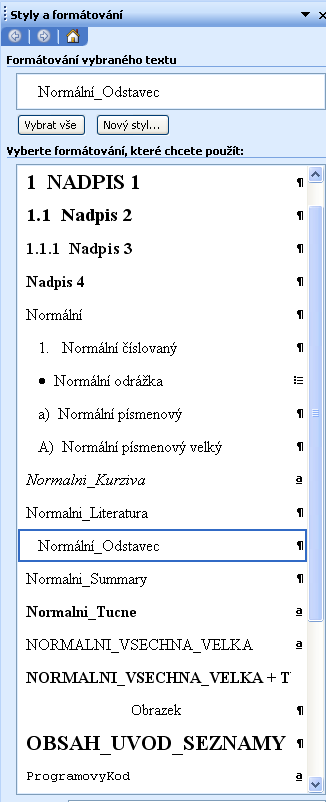
\includegraphics[width=0.2\textwidth]{./obrazky/obrazek_1.png}
      \label{fig:44}
    \end{figure}

    %ukázka odkazu na zkratky a obrázek
    \gls{Esri} \gls{SQL} bla bla bla \odkazObrazek{fig:44}. Pokud chceme uvést překlad z angličtiny můžeme to udělat takto \transl{english words}.

    %dají se dělat i složené obrázky
    \begin{figure}
        \centering
        \begin{subfigure}[b]{0.45\textwidth}
          \centering
          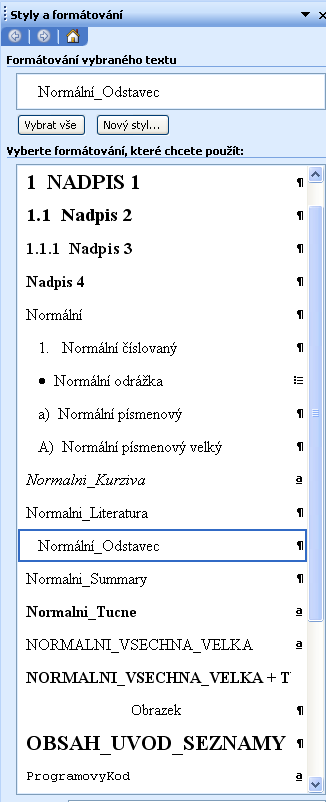
\includegraphics[width=\textwidth]{./obrazky/obrazek_1.png}
          \label{fig2.1}
        \end{subfigure}%
        \quad %add desired spacing between images, e. g. ~, \quad, \qquad etc.
          %(or a blank line to force the subfigure onto a new line)
        \begin{subfigure}[b]{0.45\textwidth}
          \centering
          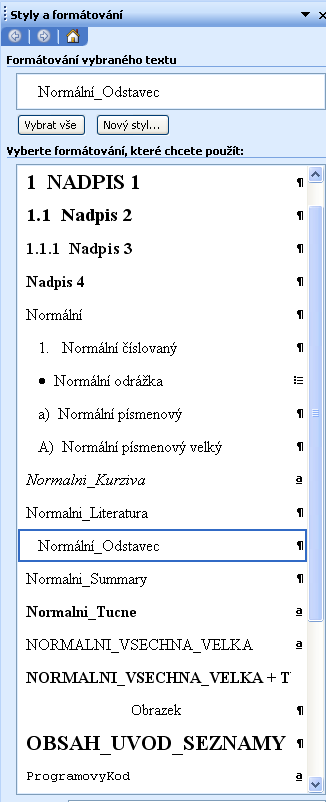
\includegraphics[width=\textwidth]{./obrazky/obrazek_1.png}
          \caption{Obsah zinku v půdě }
          \label{fig2.2}
        \end{subfigure}
        \caption{Povrch socioekonomického (a) a fyzickogeografického (b) ukazatele}
        \label{fig2}
    \end{figure}

    \begin{table}[h]
    \caption {Ukázková tabulka}
    \label{tab1}
    \centering
      \begin{tabular}{ |l|l|l| }
        \hline
        \multicolumn{3}{ |c| }{Team sheet} \\
        \hline
        Goalkeeper & GK & Paul Robinson \\ \hline
        \multirow{4}{*}{Defenders} & LB & Lucus Radebe \\
        & DC & Michael Duberry \\
        & DC & Dominic Matteo \\
        & RB & Didier Domi \\ \hline
        \multirow{3}{*}{Midfielders} & MC & David Batty \\
        & MC & Eirik Bakke \\
        & MC & Jody Morris \\ \hline
        Forward & FW & Jamie McMaster \\ \hline
        \multirow{2}{*}{Strikers} & ST & Alan Smith \\
        & ST & Mark Viduka \\
        \hline
      \end{tabular}
    \end{table}

    Odkaz na tabulku pak vytvoříme takto: \odkazTabulka{tab1}.

    \begin{equation}
    \label{eq1}
    c = \sqrt{a^2 + b^2}
    \end{equation}

    Vzorce pak odkazujeme \odkazVzorec{eq1}. 




        \subsection{Vymezení pojmů}
Pro lepší porozumění textu této práce je potřeba definovat pojmy replikace, synchronizace a verzování, včetně popisu toho, jak jsou dané pojmy chápány v produktech ArcGIS. Je vhodné upozornit, že výše zmíněné procesy jsou v literatuře často užívány lehce odlišně. Některé zdroje pojmy replikace a synchronizace rozlišují, jiné je naopak považují za synonyma. 

Všechny dotyčné pojmy úzce souvisí se zálohováním dat, tedy kopírovaním dat mezi dvěmi a více uložišti. To, co tyto pojmy spojuje, je totiž vždy, v nějaké míře, zabránění ztráty dat, ať už chybou či fyzickým poškozením disku. Dané pojmy se poté liší například konkrétním způsobem provedení zálohy, či konkrétním důvodem pro použití daného procesu.

Synchronizace je obecnější pojem, který může být považován za nadmnožinou replikace. V případě, že existují dva datové zdroje, které je potřeba v daný okamžik sjednotit, je možno mluvit o synchronizaci souborů či datových složek. U souborů se shodným názvem se porovnává čas posledního zápisu, velikost nebo obsah souboru, naopak soubory, které shodu nezaznamenají, jsou jednoduše zkopírovány. Synchronizací se tedy dá proces označit v okamžiku, kdy existují nejméně dva datové zdroje a smyslem synchronizace je porovnat tato uložiště a dostat je do stejného stavu. To může například přispět snazší spolupráci více uživatelů nad stejnými daty nebo uživateli, který pracuje na více počítačích.


        %parametr H říká že to bude přímo na tom místě kde je v textu...více http://en.wikibooks.org/wiki/LaTeX/Floats,_Figures_and_Captions
          \begin{figure}[H]
            \centering
            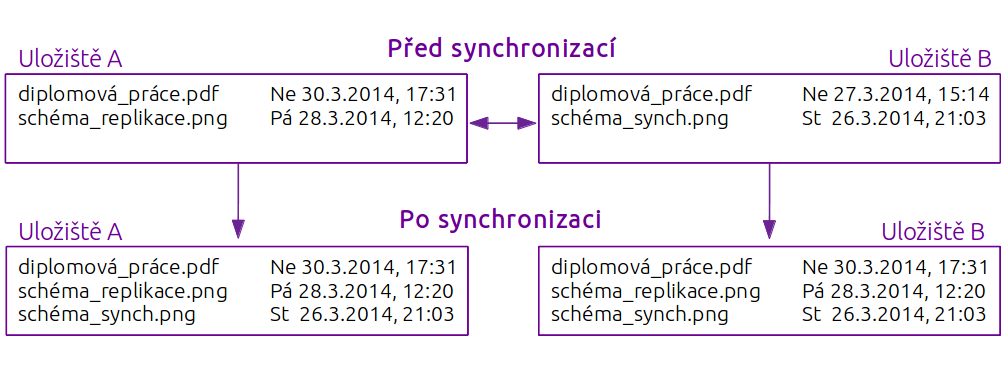
\includegraphics[scale=1]{../../../grafy/obr/schema_synchronizace_maxiTence.png}
            \caption {Příklad obousměrné synchronizace dat mezi dvěmi datovými uložišti}
          \end{figure}

Replikace naopak začíná s daty existujícími pouze na jednom uložišti. Často je tento proces používán právě ve spojitosti s databázemi, kdy je kopie dat (také replika) tvořena z důvodu snížení zátěže serveru, či ochraně dat. Replikace je tedy často vyžadována z jiných důvodů než synchronizace a pro zajištění konzistence dat používá jiných technologií. V případě, že je již kopie vytvořena, je poté možno mluvit i o synchronizaci dat, protože replika průběžně kontroluje, zda na hlavním serveru nedošlo ke změně, a pokud ano, dané změny zkopíruje. Více se replikací zabývá kapitola \odkazKapitola{kReplikace} Replikace.

Oba procesy je možno použít jednostranně, tedy kopírovat data pouze z jednoho uložiště na druhé a nikolik opačně, nebo oboustraně, kdy se datové zdroje kopírují navzájem mezi sebou.

Specifickým způsobem zálohy dat je verzování, kdy se data na záložním datovém uložišti nepřepisují, ale systematicky ukládající v takzvaných verzích tak, aby se uživatel mohl snadno kdykoliv vrátit k předchozím stavům souborů. Smyslem verzování je zachovat všechny zvolené stavy práce, čímž se verzování liší od zálohování, kde stačí mít aktuální kopii daných dat. To, co je zde popsáno jako verzování, se v produktech ArcGIS nazývá archivování dat \citep{Law2008}. 

Verzování může probíhat ručně, poloautomatizovaně či plně automatizovaně díky speciálním nástrojům pro správu verzí, kterých je na internetu dostupná celá řada. Oblíbeným verzovací systémem programátorů je Git\footnote{více na http://git-scm.com/}, open-source nástroj pro správu verzí, který pomáhá při práci s malými i velkými projekty a podporuje týmovou spolupráci. Umožňuje vrátit jednotlivé soubory nebo celý projekt do předchozího stavu, porovnávat změny provedené v průběhu času, zjistit, kdo naposledy upravil něco, co nyní možná způsobuje problémy, kdo vložil jakou verzi a mnoho dalšího \citep{Chacon2009}. Git je vhodný zejména pro textové soubory, protože dokáže analyzovat části textu, či programového kódu a zvýraznit místa, která se změnila.
        
          \begin{figure}[H]
            \centering
            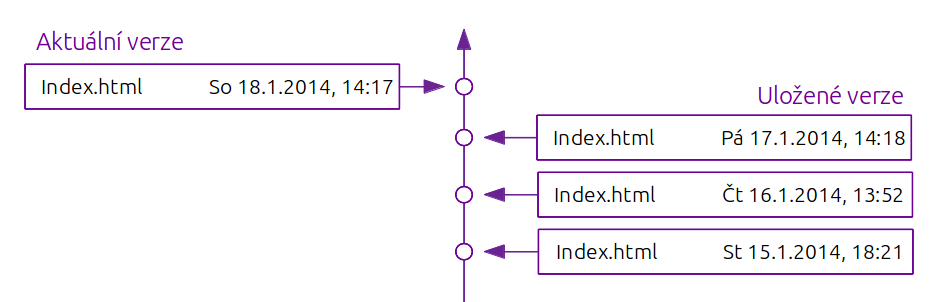
\includegraphics[scale=1]{../../../grafy/obr/schema_verzovani_maxiTence.png}
            \caption {Příklad verzování souboru}
          \end{figure}

Samotná databáze verzování dat neumožňuje. Nejsnazší způsob, jak získat verzi dat, je skriptem \texttt{dump}, který exportuje databázi do souboru. V MS SQL Serveru je tento proces nazýván Snapshot, tedy snímek databáze nebo také snímková replikace. Takový soubor se poté může verzovat podobným způsobem jako jakýkoliv jiný binární soubor typu shapefile. A to samé platí i pokud v databázi ukládáme geodata. 

Proto byl vytvořen verzovací systém také pro prostorová data, který vychází ze systému Git a nese název GeoGIT. Umožňuje uživatelům uchovávat změny v souborech shapefile, SpatialLite a z databáze PostGIS (PostgreSQL), stejně tak jako vrátit se k jakékoliv z předchozích verzí. 

Verzování může být chápáno také jako vytvoření pracovní verze. V případě, že programový kód či data jsou plně funkční či správná, ale je potřeba je aktualizovat, testovat či jinak měnit, pak je vhodné vytvořit tzn. pracovní verzi, aby nedošlo k poškození té aktuální. Jedná se o kopii aktuálního stavu, na které je možno pracovat a zkoušet. V případě, že práce nedopadne podle představ, je možno změny zahodit, pokud je tomu naopak, je možno pracovní verzi sjednotit s platnou verzí. Tento způsob verzování umožňuje Git i GeoGIT a takto chápe pojem verzování i společnosti Esri.

          \begin{figure}[H]
            \centering
            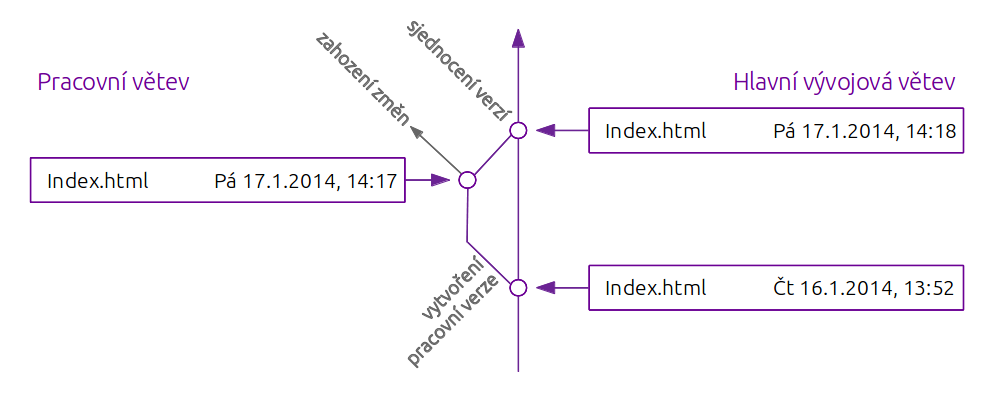
\includegraphics[scale=1]{../../../grafy/obr/schema_verzovaniBranch.png}
            \caption {Příklad verzování souboru s použitím pracovní větve}
          \end{figure}

        


        \subsection{Replikace}
        \label{kReplikace}
Replikace je proces, u kterého jsou data a databázové objekty kopírovány z jednoho databázového serveru na druhý a poté synchronizovány pro zachování souladu obou databází. Synchronizací v tomto případě myslíme kopírování všech změn, které v databázi nastanou. Použitím databáze je možno data distribuovat na různě vzdálená místa nebo mezi mobilní uživatele v rámci počítačové sítě a internetu \citep{Microsoft2013}.

Mnohé moderní aplikace se musí zabývat velkým počtem současných přístupů do databáze, což může v některých případech způsobovat problémy. Buď je server přetížen počtem připojení a data tedy přicházejí k uživateli pomalu, nebo dokonce úplně vypadne. 

Mezi časté důvody použití databázové replikace tedy patří zajištění dostupnosti dat\footnote{angl. High Availability}, resp. snížení pravděpodobnosti, že data nebudou dostupná, což může být způsobeno již zmíněným výpadkem serveru nebo například fyzickou ztrátou dat \citep{ObeHsu2012}. Další důvodem je rozložení zátěže přístupů do databáze mezi více serverů, takže nebude docházet ke zpomalení výkonu hlavního serveru ani k situaci, že data nebudou dostupná kvůli jeho výpadku \citep{BellKindahlThalmann2010}. Databáze je často zálohovaná, například skriptem dump a i to může server zpomalit. Vhodným řešením je tedy nejdříve vytvořit kopii dat na jiný datový server a až poté proces zálohování spustit. 

Všechny databáze zapojené do procesu replikace jsou v odborné literatuře nazývané uzly, angl. node. Tyto uzly dohromady tvoří replikační cluster\footnote{volně přeloženo jako skupina serveru zapojených do replikace}. Při správně nastavené replikaci, jejímž cílem je zajištění vysoké dostupnosti dat (HA), by v clusteru nikdy neměly být méně než tři uzly. Může se totiž stát, že vypadne jeden ze dvou uzlů, čímž dojde, ikdyž jen na krátkou chvíli, k situaci, že data nebudou v daný okamžik zálohovaná. 

Uzly v replikačním clusteru mohou mít jednu ze dvou základních rolí, nejčastěji nazývaných master a slave. Master server nebo pouze master je server, který poskytuje data k replikaci, má práva na čtení i zápis a probíhají tedy na něm veškeré aktualizace. Je možno se setkat také s pojmenováním Primary server, Provider, Sender, Parent nebo Source server. Naprosto jiný pojem zavádí SQL Server, který tento zdrojový server nazývá Publisher (česky Vydavatel). Druhý databázový server je nejčastěji nazýván slave, Standby, Reciever, Child nebo Subsciber (česky Odběratel). Poslední pojem je také používán SQL Serverem. Na tento server, který je dostupný vždy jen pro čtení dat, se data a aktualizace kopírují, není však možné na něj změny zapisovat \citep{RiggsKrossing2010}.

        %parametr H říká že to bude přímo na tom místě kde je v textu...více http://en.wikibooks.org/wiki/LaTeX/Floats,_Figures_and_Captions
          \begin{figure}[H]
            \centering
            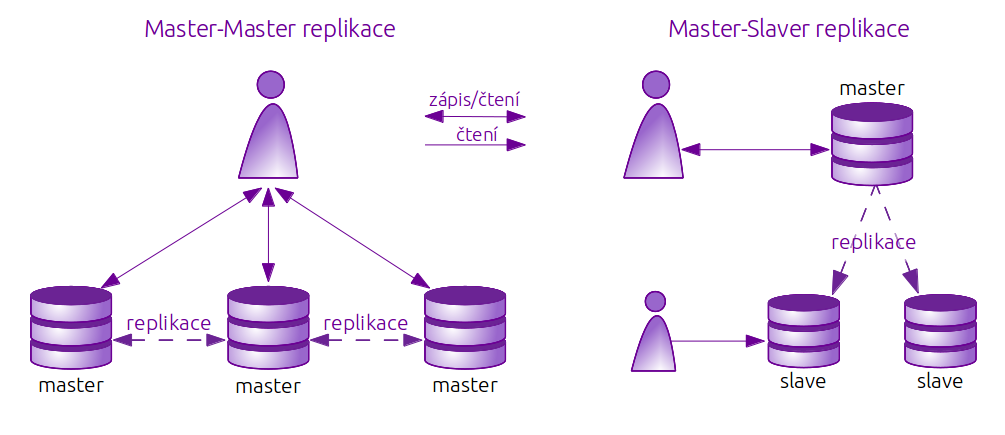
\includegraphics[scale=1]{../../../grafy/obr/schema_masterMasterSlave.png}
            \caption {Srovnání Master-Master a Master-Slave replikace}
            \label{srovnaniM-M-S}
          \end{figure}

Podle počtu master a slave serverů v replikačním clusteru, se rozlišuje zda se jedná o jednosměrnou nebo obousměrnou replikaci. Tzv. master-master replikace umožňuje zapisovat do všech uzlů v replikačním clusteru, což může být praktické například při použití databáze offline \odkazObrazek{srovnaniM-M-S}. Změny se tedy synchronizují mezi všemi databázovými uzly. Tento způsob však nese značné komplikace, je potřeba řešit konflikty změn ve stejných datech a je relativně náročný na údržbu. Tato práce se zabývá použitím druhé způsobu, tzv master-slave replikace. Tato replikace používá vždy jen jeden master server v clusteru a dva a více slave servery. Kopie dat tedy probíhá jednosměrně, vždy z master na slave servery. Podle Bella a kol. (2010) mají moderní aplikace často více čtenářů než zapisovatelů, proto je zbytečné, aby se všichni čtenáři připojovali na stejnou databázi jako zapisovatelé a zpomalovali tím jejich práci \citep{BellKindahlThalmann2010}. Z toho důvodu je tedy použití master-slave replikace více než vhodné.

Při návrhu replikace je potřeba se zamyslet také nad tím, zda bude synchronní či asynchronní. Synchronní replikace neumožní potvrzení transakce modifikující data, dokud všechny změny nejsou přeneseny na slave server \citep{Boszormenyi2013}. Tento přístup zajistí, že žádná data nebudou v průběhu transakce ztracena. V některých případech tento způsob může zbytečně zpomalit rychlost přístupu do databáze, protože je nutno čekat na každou nedokončenou transakci. Zároveň může způsobit snížení dostupnosti databáze, protože v případě, že se například přeruší spojení mezi servery, nemůže být na master serveru potvrzena žádná další transakce. Ale jistě si najde své opodstatění například při bankovních transakcích, kde je potřeba, aby všechny operace proběhly na obou stranách. V tomto případě je užití tohoto způsobu zcela nezbytné. 

Druhým způsobem je asynchronní replikace, při které se nová data mohou zapisovat na master server, přestože ještě nedošlo k replikaci stávajících dat na slave server \citep{ObeHsu2012}. To je sice za běžného provozu rychlejší, v některý případech však může způsobit nekonzistenci dat, například když proběhne transakce na master serveru, který však spadne dřív, než se změna zapíše na slave. V takovém případě se slave změní na master server, ale zároveň se nikdy nedozví o transakci, o které má uživatel informace, že proběhla v pořádku. 

        \begin{figure}[H]
          \centering
          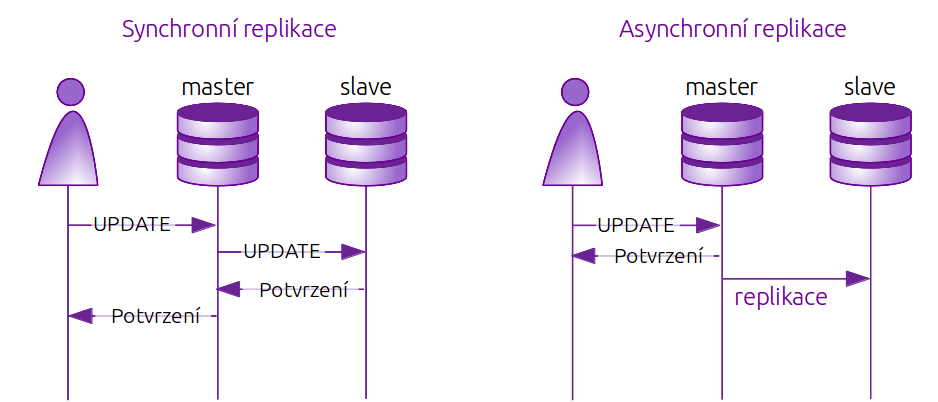
\includegraphics[scale=1]{../../../grafy/obr/schema_asyncSync_maxiTence.png}
          \caption {Rozdíl mezi synchronní a asynchronní replikací}
        \end{figure}
Replikace v PostgreSQL umožňuje plnou kopii dat z databáze i pouze výběr některých tabulek. Více o možnostech a způsobech nastavení replikace v kapitolách \odkazKapitola{kPriprava} Příprava prostředí pro konfiguraci a \odkazKapitola{kKonfigurace} Konfigurace replikace.

Dále je možno rozlišovat replikaci pole toho, zda je logická nebo fyzická. Fyzická replikace na druhý server kopíruje bloky binárních datových souborů bez znalosti jejich struktury (sloupce, řádky, …), čímž se zajistí identická replika. Pro tento způsob kopírování dat, která mají jasně danou strukturu, je potřeba mít na obou serveru stejnou platformu a architekturu. Tento způsob je velice spolehlivý a často snazší na konfiguraci. 

Naopak logická přenáší data v textové podobě, která nese informace o příkazu a struktuře. Tento způsob je více flexibilní, umožňuje výběr jen několika databází nebo tabulek a není závislý na architektuře ani operačním systému \citep{Boszormenyi2013}. 

Posledním diskutovaným pojmem je kaskádová replikace, která umožňuje připojit repliku k jinému slave serveru místo k hlavnímu master serveru. Tento způsob může být výhodných předeším z těchto dvou důvodů. Řekněme, že se kaskádová replikace použivá při existenci většího počtu slave serverů v clusteru, třeba sta. V případě, že by se všechny repliky připojovaly k hlavnímu serveru, došlo by u něj k razantnímu zpomalení jeho výkonu. Kaskádová replikace může být praktická také v okamžiku, kdy se data přenáší na velkou vzdálenost, třeba do Číny. V případě, že mají v Číně dvě repliky, je zcela zbytečné, aby se obě kopie přenášely na tak velkou vzdálenost, když druhá replika se může připojit k první a mít data s mnohem menším zpožděním.

          \begin{figure}[H]
            \centering
            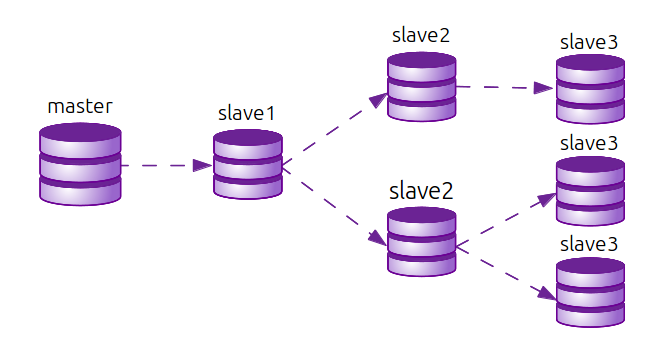
\includegraphics[scale=1]{../../../grafy/obr/schema_kaskadova.png}
            \caption{Ukázka kaskádové replikace}
            \label{kaskadova}
          \end{figure}

Každý databázový server (myšleno SŘDB) si volí terminologii a konkrétní nastavení mírně odlišně. Tato kapitola se snaží popsat chápání replikace co v největší míře obecně s ohledem na použití tohoto pojmu v PostgreSQL. Zcela jinou terminologii, ikdyž založenou na stejných principech, zavádí SQL Server, který pro export databáze do souboru používá pojem snímková replikace, pro master-slave replikaci pojem transakční replikace a pro master-master replikaci slučovací replikace. 




Tato kapitola se zabývá hodnocením současného stavu správy dat na katedře geoinformatiky, návrhem databázového řešení dle požadavků a možností katedry a podrobně popisuje vytvoření testovacího prostředí na serverech katedry dle vytvořeného návrhu. Do hloubky popisuje konfiguraci vybraných nástrojů, včetně jejich nasazení.

Katedra má zájem využít potenciál databázového řešení, které bude zajišťovat efektivní uložení, sdílení a správu dat, která má katedra k dispozici. Zároveň má v~plánu vyučovat problematiku správy dat v~databázi. Studenti se budou moci nejen dozvědět o způsobech uložení dat, ale také je prakticky vyzkoušet, pochopit jejich fungování, naučit se pracovat s daty nahranými do GIS software a v neposlední řadě tato data použít pro své projekty a závěrečné práce. Velkou výhodou bude také větší připravenost do praxe, kde je databázové ukládání dat hojně rozšířeno. Data uložená v~databázi pak budou mnohem snáze využitelná jak pracovníky katedry, tak i jejími studenty. 

\subsection{Aktuální stav správy dat}
\label{kAktualniStav}

Katedra aktuálně provozuje tři servery, konkrétně \texttt{virtus.upol.cz}, \texttt{atlas.upol.cz} a~\texttt{geo\-hydro.upol.cz}. Poslední z jmenovaných byl poskytnut jako testovací server pro tuto práci a v budoucnu se s ním počítá jako s master serverem pro zde popisované databázové řešení. První dva zmíněné servery jsou aktivně používány, hostují například geoportál publikovaný skrze ArcGIS Server, který je důležitým prostředkem pro prezentaci projektů a dat, která na katedře vznikají. Data ke geoportálu i dalším aplikacím běžícím na těchto serverech jsou ukládána do MS SQL Serveru, přičemž každý ze serverů obsahuje jiné datové sady, které nejsou pravidelně zálohovány, protože jejich aktualizace není příliš častá. Aktuální řešení nepoužívá replikaci dat, data tedy mohou být nedostupná z důvodu výpadku serveru. 

Databáze aktuálně obsahují data například z projektů BotanGIS\footnote{\url{http://botangis.upol.cz/botangis/mapa}}, Virtuální studovna CHKO Litovelské Pomoraví\footnote{\url{http://virtus.upol.cz/}}, dále data metadatového systému Micka\footnote{\url{gislib.upol.cz/metadata}}, data ze senzorové sítě KGI, data ke studentským pracím a také ukázková data určená pro výuku. Je založeno přibližně 10 účtů, které mají přístup pro zápis, a řádově v desítkách účtů s právem čtení, do databází aktuálně není příliš často zapisováno. 

Velké množství dat, které má katedra k dispozici, je však stále uloženo ve formátech Shapefile nebo File Geodatabase. Každý kdo chce tato data použít, musí je přenést přes různá hardwarová zařízení nebo je zkopírovat po síti. Studenti si musejí dělat kopie dat při každém cvičení, což velice zdržuje výuku. Často se totiž jedná o velké objemy dat, jejichž kopie může trvat řádově v jednotkách až desítkách minut. Data jsou poté fyzicky uložena na počítačích v učebnách, což mimo jiné dovoluje, aby se k datům dostal kdokoliv, kdo má na učebnu přístup. Není tedy přehled o tom, kdo data využívá. Studenti navíc netuší, s jakými daty pracují a nabývají nesprávných představ o tom, že všechna data jsou vždy uložená ve formátu Shapefile. Zároveň se špatně zajišťuje aktualizace dat, při které, není-li spravována centralizovaně, může docházet k nekonzistenci dat. Při kopírováním dat na různá datová uložiště je navíc těžké dodržet licenční podmínky, se kterými jsou data pořizována. 

\subsection{Požadavky na databázové řešení}
\label{kPozadavky}

Základním požadavkem byl výběr takového databázového systému, který je široce používán v oblasti geoinformatiky a zároveň je podporován produkty ArcGIS. Požadavem bylo také zhodnocení finanční stránky, replikace je totiž v mnohých komerčních systémech zařazena až mezi nejpokročilejší funkcionalitu a tedy je dostupná až s drazšími licencemi. 

Katedra má v zájmu ukládat do databáze mnohem více datových sad, které má k dispozici a které jsou momentálně dostupné pouze ve formátech Shapefile nebo File Geodatabase. Jedná se například o datové sady ArcČR500 verze 2.0 a 3.0, Data200 (ČUZK), CEDA ČR 150, data, která byla uvolněna jako podpora pro Krajinotvorný program MŽP, nebo data dostupná k produktům Esri nebo Idrisi. Databázové řešení by tedy mělo být navrženo tak, aby uneslo mnohem větší počet připojení a dotazů než v současné době, protože datového sady, které budou nově dostupné skrze databázi, budou používány v řadě cvičení. Plánem je v rámci cvičení studentům umožňit plnohodnotnou práci s daty, tedy povolit jim jak čtení dat, tak zápis do databáze. 

Návrh by měl také zohlednit zájem katedry o využití jednoho ze serverů jako slave server pro replikaci dat ze senzorové sítě Ekodata. 


\section{Návrh replikačního řešení}
  Po provedení rešerše a zohlednění všech podmínek, požadavků a možností
  katedry, byl sestaven návrh kompletního databázového řešení založeného na
  procesu replikace. Z databázových serverů byl vybrán server PostgreSQL hned
  z~několika důvodů. Jedná se o plnohodnotný databázový systém dostupný zda\-rma
  se všemi nástroji, je široce používaný v oblasti geoinformačních technologií,
  je multiplatfomní a od verze ArcGIS 9.3 plně podporováný produkty ArcGIS.
  Návrh počítá s použitím ArcSDE pro propojení databáze s ArcGIS produkty. Při
  výběru verzí je nutné zajistit kompatibilitu verzí jednotlivých software,
  a~poté ArcSDE nainstalovat společně s PostrgreSQL.

  Byl navržen replikační cluster s nejméně třemi servery z důvodů, které již
  byly diskutovány v kapitole \ref{kReplikace}. Celý cluster poběží na stejné
  platformě a proto bude možno použít streaming replikaci se všemi výhodami
  zmíněnými v kapitole \ref{kReplikace}. Byla zvolena jednosměrná master-slave
  replikace, cluster tedy bude obsahovat jeden master a dva (popř. více) slave
  serverů. Aby nedošlo ke ztrátě dat v~případě, že by master server spadl dřív,
  než se data zkopírují na slave server, pro první slave (\texttt{slave1}) byla
  zvolena varianta synchronní replikace. Je vhodné, aby servery běžely
  v~lokální síti z důvodu rychlosti a spolehlivosti spojení mezi master a slave
  serverem. 


  Druhý server (\texttt{slave2}) bude replikovat asynchronně a zároveň, aby
  ne\-do\-chá\-ze\-lo k~přetížení master serveru, bude replikace probíhat ze
  \texttt{slave1} na \texttt{slave2}, tedy kaskádově. Tím bude řešení zároveň
  přípraveno na výpadek master serveru, protože v~případě, že master vypadne,
  \texttt{slave1} bude povýšen na master a \texttt{slave2} bude ihned moci
  replikovat. Ze \texttt{slave2} lze dále tvořit pravidelnou, například denní
  nebo týdenní, zálohu pomocí ulitily \texttt{pg\_dump}. Záloha pomocí
  \texttt{pg\_dump} tak nebude zatěžovat master server a sama o sobě bude
  probíhat rychleji, než by tomu bylo na master serveru, který je již tak velmi
  vytížen dalšími procesy.

  \begin{center}
    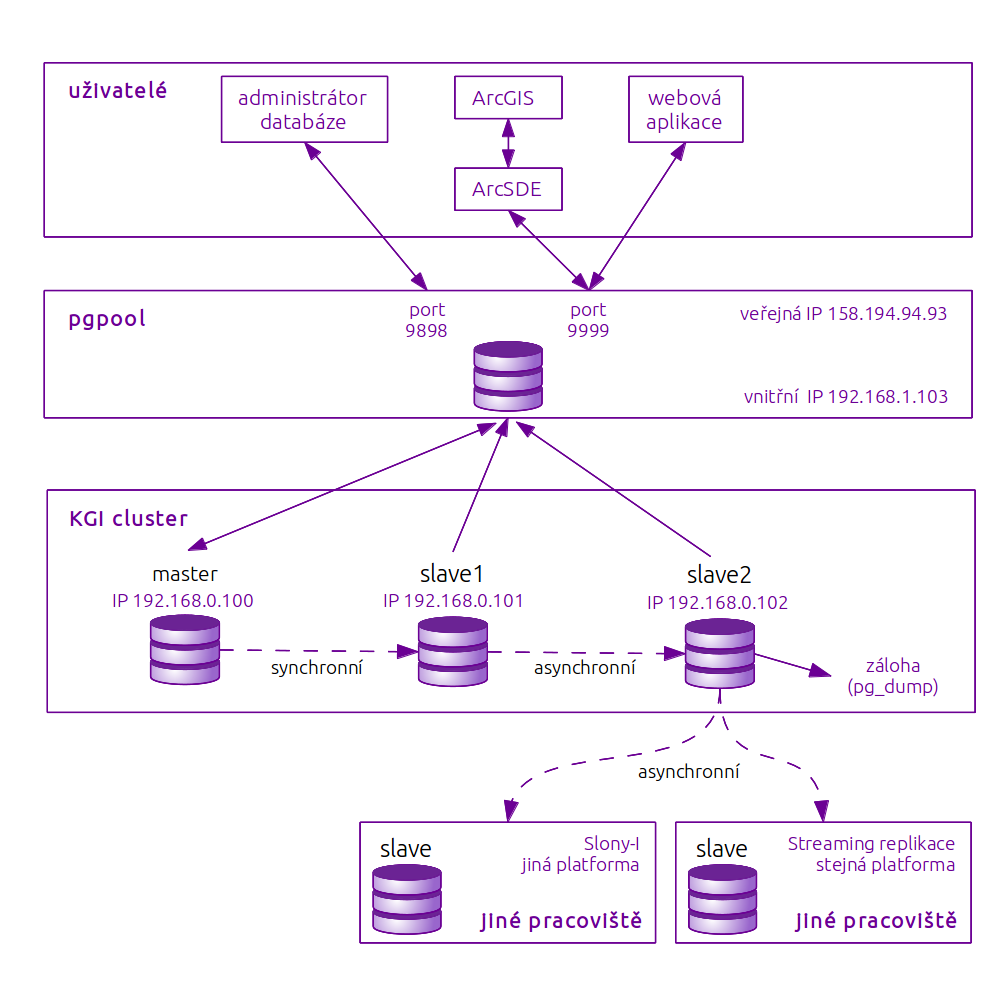
\includegraphics[width=\textwidth]{obr/schema_navrhKatedra.png}
       Srovnání multimaster a master-slave replikace
  \end{center}

Uživatelé se budou připojovat skrze nástroj pgpool, který se bude tvářit jako jediný databázový server, ke kterému se klienti přihlásí bez ohledu na typ jejich dotazu a on sám pak rozhodne, ke kterému ze serverů klienta přihlásí. Tím bude mít zároveň možnost rozložit zátěž na dostupné uzly v clusteru. Pro ještě větší efektivitu provozu databáze bude pgpool uchovávat databázová spojení a při novém dotazu využije stávajícího spojení, místo aby vytvářel spojení nové. 

Vzhledem k tomu, že klienti budou k databázovému serveru přistupovat skrze pgpool, není potřeba aby jednotlivé uzly v clusteru měly veřejnou IP adresu. Plně dostačuje, že servery poběží na lokální síti a pouze pgpool bude na serveru s veřejnou IP, čímž se zajistí, že data budou přístupná z internetu. 

Návrh počítá také s externími pracovišti, která budou často číst z databáze a~budou mít zájem o zrychlení přístupu k datům tím, že se slave server přesune na jejich pracoviště. Typ replikace se zvolí podle jejich operačního systému a jeho architektury. Pokud se bude jednat o shodný systém, jaký bude použit ve výše popsaném clusteru, pak bude možno použít asynchronní streaming replikaci, naopak pokud se bude jednat o systém jiný, bude použita Slony-I replikace. 



\begin{thebibliography}{99}
    \bibitem{Oppel2009} OPPEL, A. J. \emph{Databases: A Beginner’s Guide}. New York: McGraw-Hill, 2009, 164 s. ISBN 00-716-0846-X.
\bibitem{Connolly2005} CONNOLLY, T. \emph{Database Systems: A Practical Approach to Design, Implementation, and Management}. Vyd. 4. Harlow: Addison-Wesley, 2005, 1374 s. ISBN 03-212-1025-5.
\bibitem{Momjian2001} MOMJIAN, B. \emph{PostgreSQL: Introduction and Concepts}. Boston, MA: Addison-Wesley, 2001, xxviii, 461 s. ISBN 02-017-0331-9.
    \bibitem{Microsoft2013} MICROSOFT. SQL Server - Replication. \emph{Microsoft} [online], 2013 [cit. 2013-08-27]. Dostupné z: http://technet.microsoft.com/en-us/library/ms151198(v=sql.100).aspx.
    \bibitem{ObeHsu2012} OBE, R., HSU, L. \emph{Postgresql: Up and Running}. Sebastopol, CA: O’Reilly, 2012, 164 s. ISBN 978-144-9326-333.
    \bibitem{BellKindahlThalmann2010} BELL, C., KINDAHL, M., THALMANN, L. \emph{MySQL High Availability}. Vyd. 1. Sebastopol, CA: O’Reilly Media, Inc, 2010. ISBN 978-059-6807-306.
    \bibitem{RiggsKrossing2010} RIGGS, S., KROSING, H. \emph{PostgreSQL 9 Administration Cookbook: Solve real-world     PostgreSQL problems with over 100 simple, yet incredibly effective recipes}. Birmingham: Packt Publishing, 2010, 345 s. ISBN 978-1-849510-28-8.
    \bibitem{Boszormenyi2013} BÖSZÖRMENYI, Z., SCHÖNIG, H.-J. \emph{PostgreSQL Replication: Understand basic replication concepts and efficiently replicate PostgreSQL using high-end techniques to protect your data and run your server without interruptions}. Vyd. 1. Birmingham: Packt Publishing, 2013, vii, 230 s. ISBN 978-1-84951-672-3.

\end{thebibliography}

\end{document}
